\documentclass[tikz]{standalone}
\begin{document}
\noindent
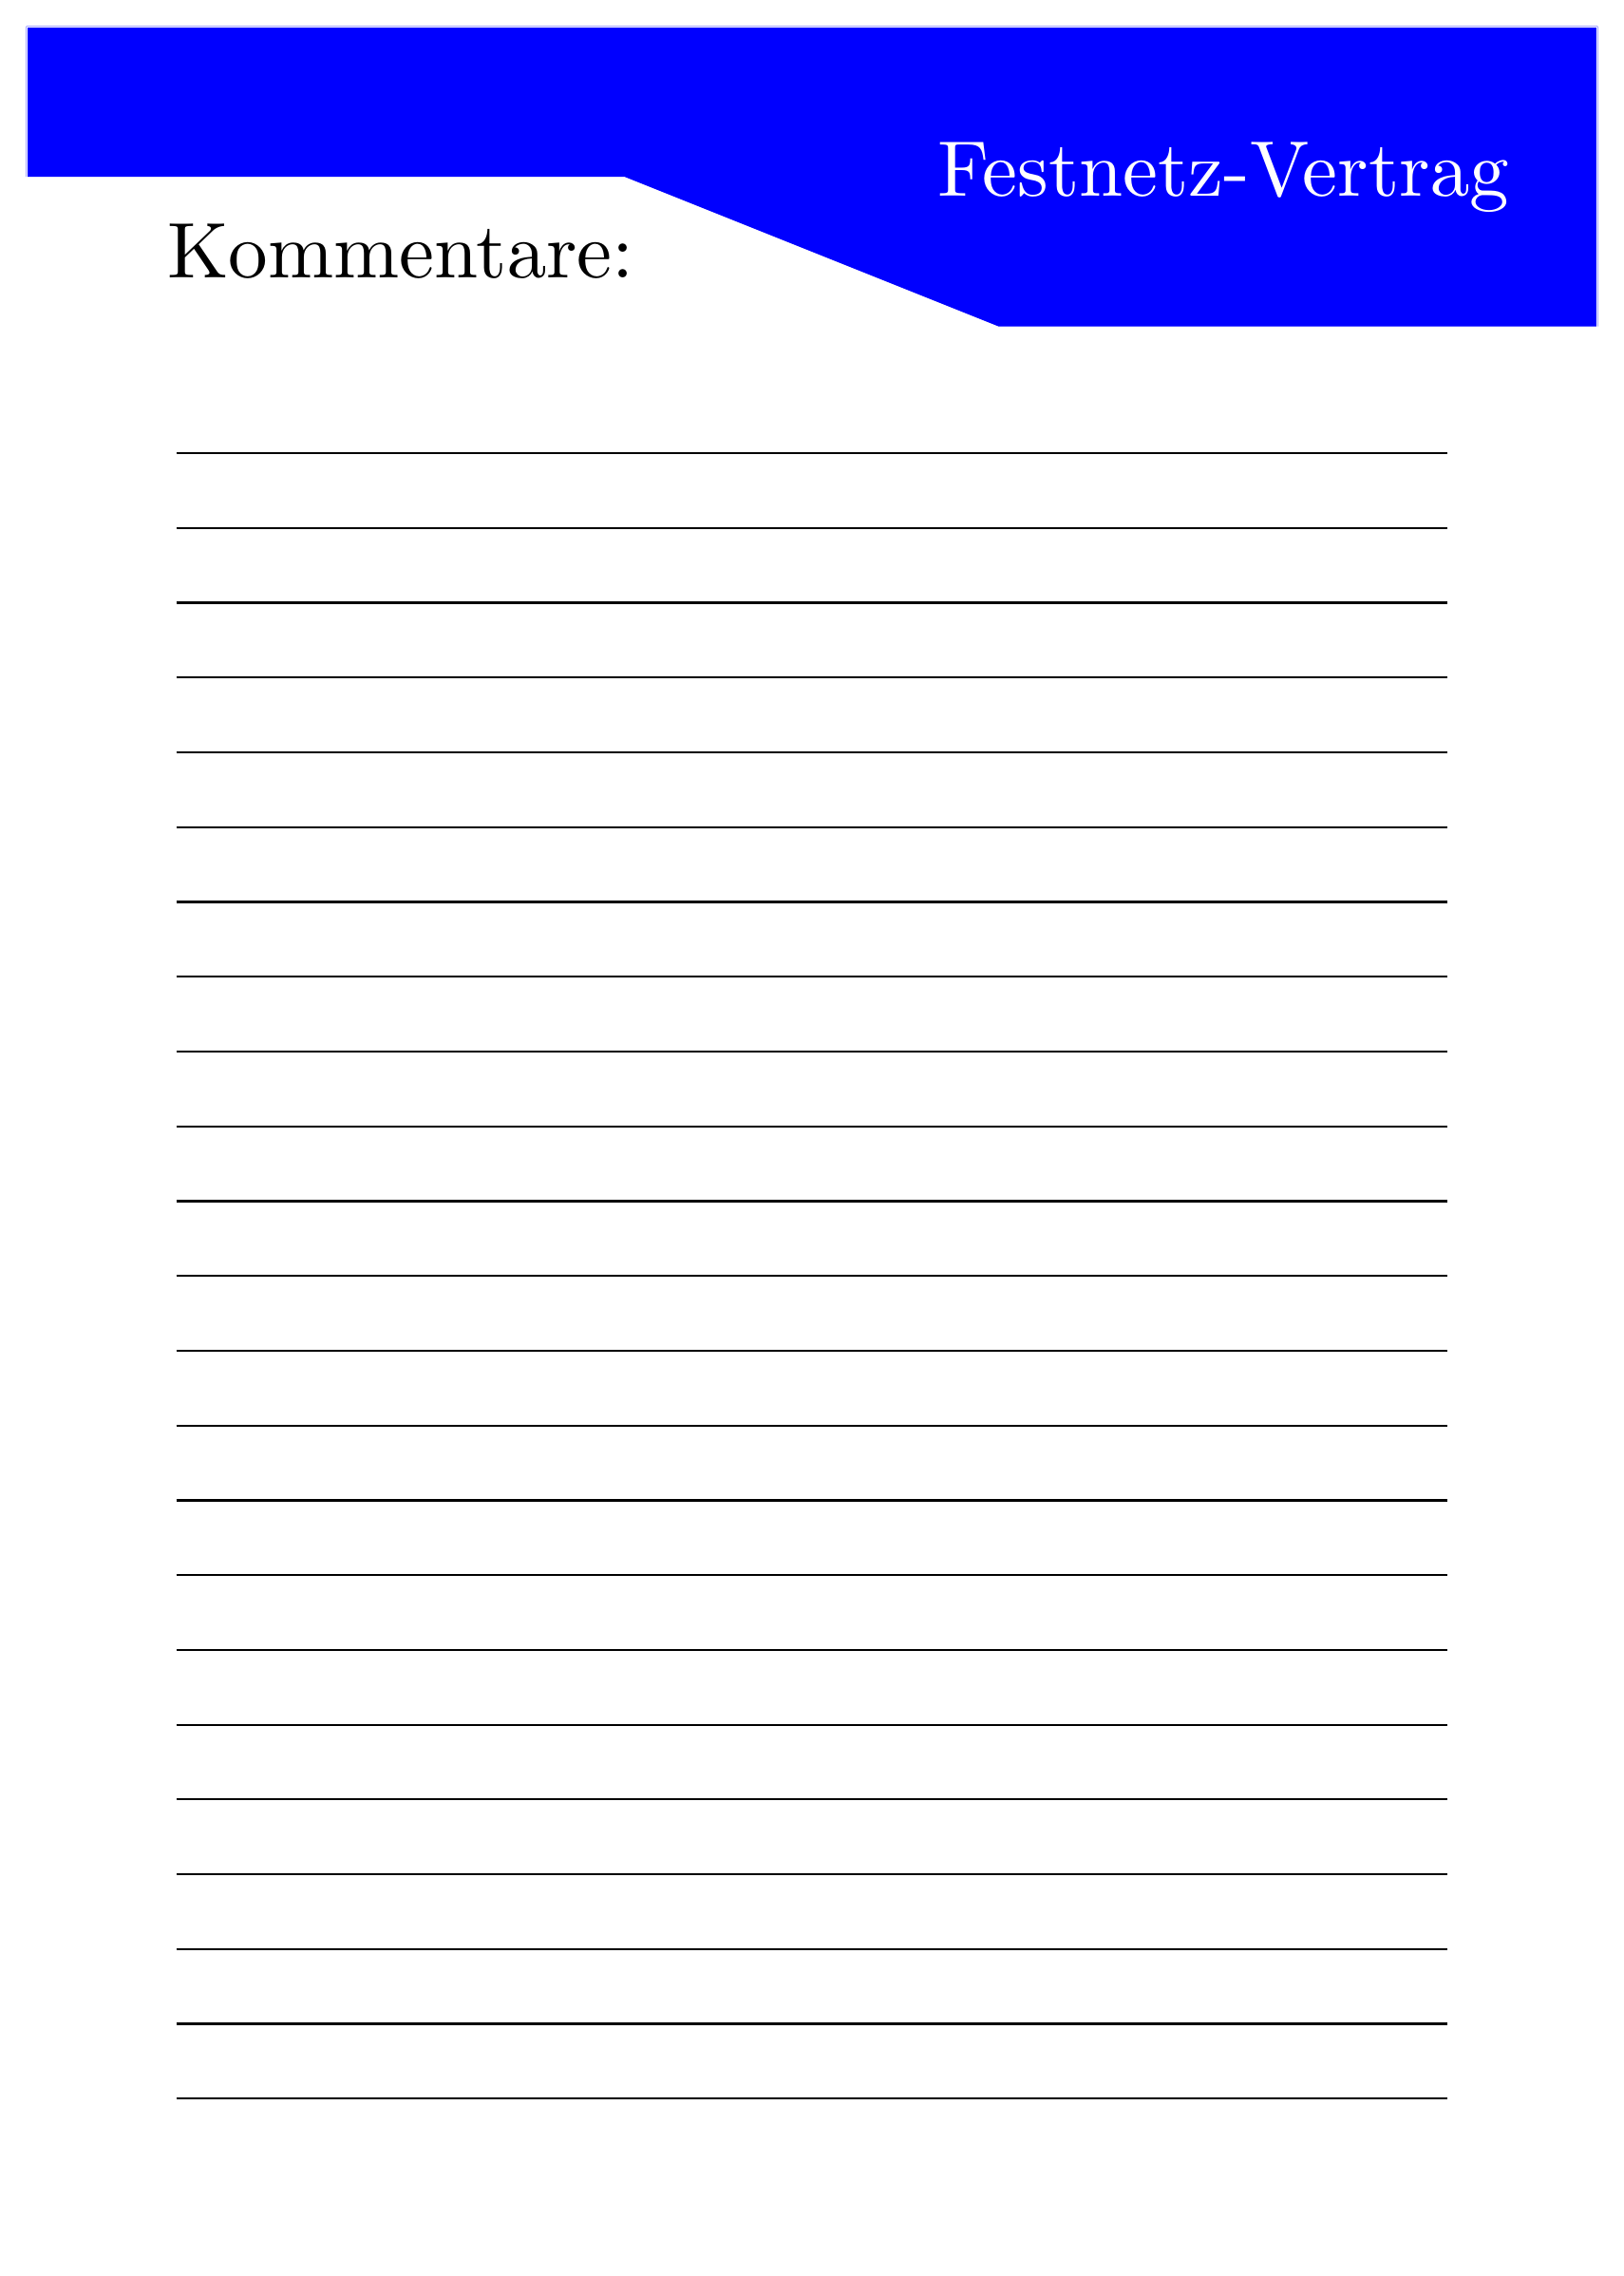
\begin{tikzpicture}

  % Decoration
  \draw[color=blue, fill=blue] (0,29.7) -- (0,27.7) -- (8,27.7) -- (13,25.7) -- (21,25.7) -- (21,29.7) -- cycle; 

  \node[thick, scale=3, align=center, color=white] at (16, 27.7) {Festnetz-Vertrag};

  % Background
  \draw[color=white] (0,0) -- (0,29.7) -- (21, 29.7) -- (21, 0) -- cycle;

  \foreach \x in {0,1,...,22}
    \draw[thick] (2,24 - \x) -- (19,24 - \x);

  % Kommentare
  \node[thick, scale=3, align=center] at (5, 26.7) {Kommentare:};

  \end{tikzpicture}%
\end{document}
